% vim: ts=2:sw=2:tw=80:et
\thispagestyle{fancy}
\pagestyle{fancy}


\begin{figure}[hb!]
  \centerline{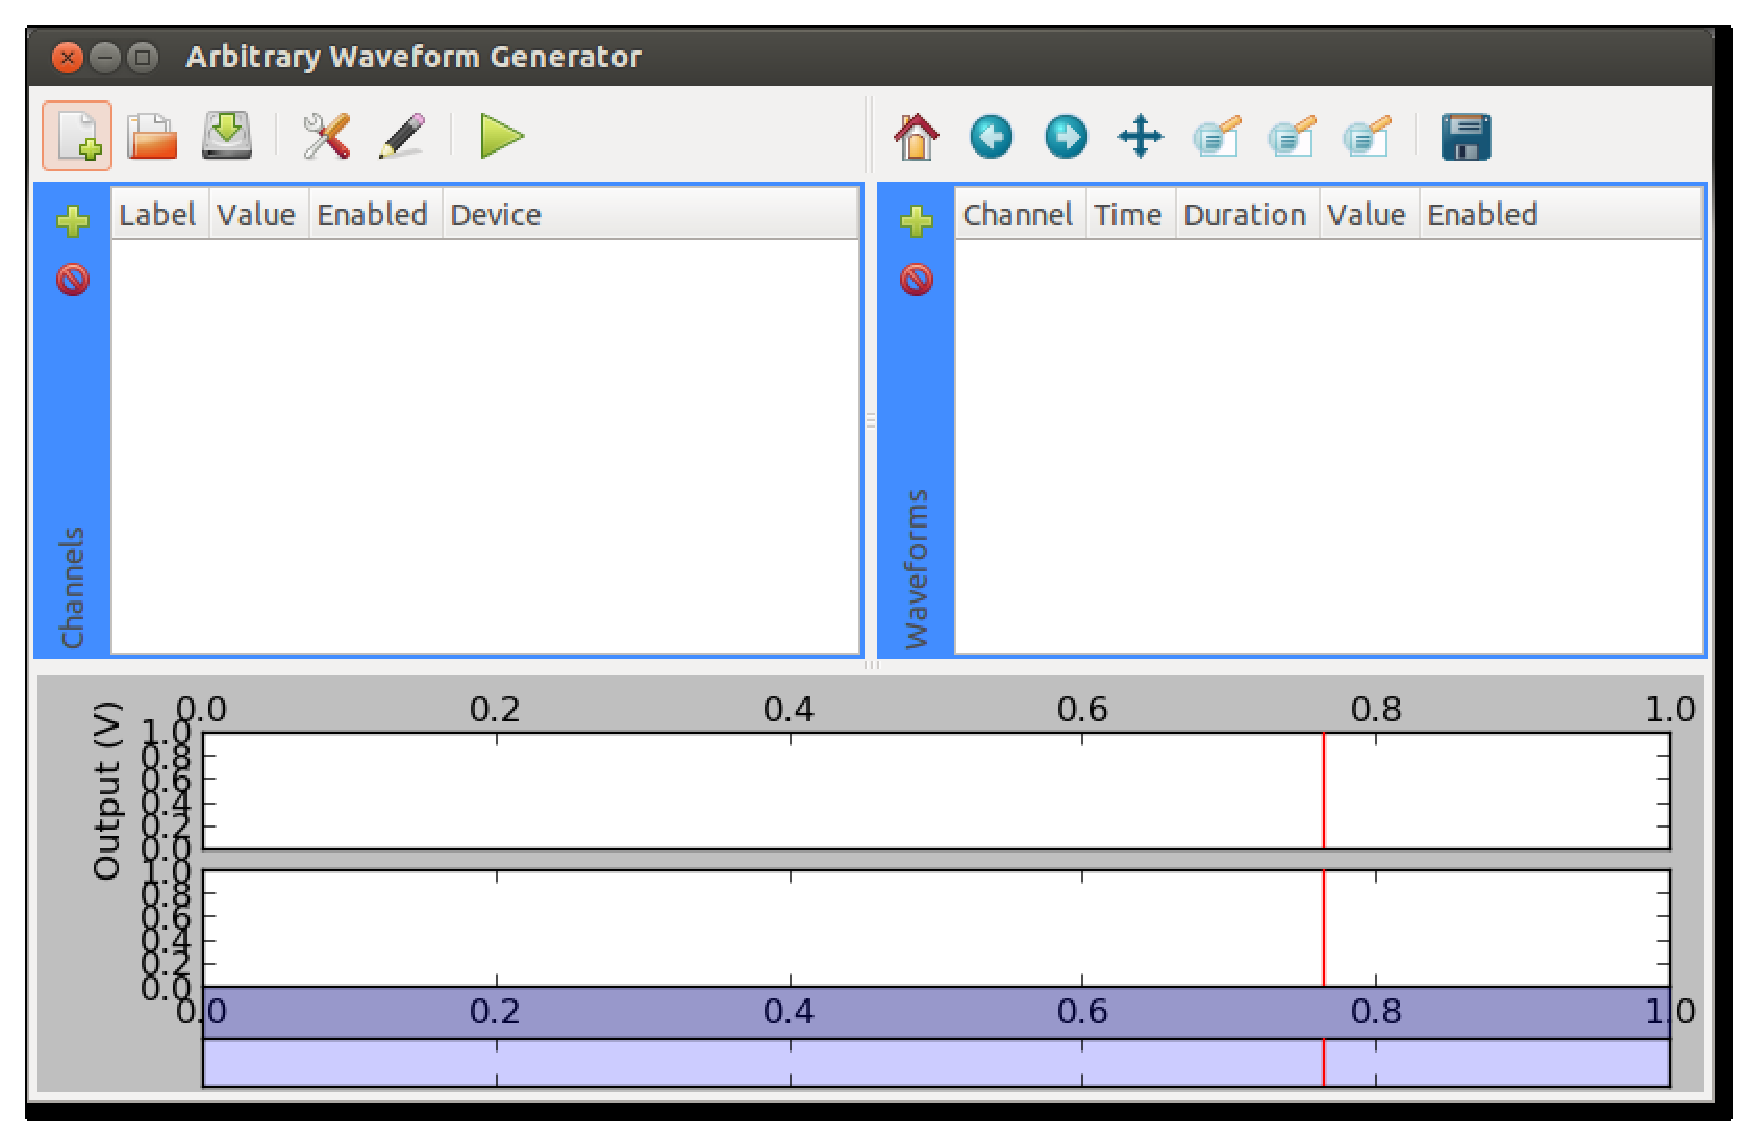
\includegraphics[width=\textwidth]{figures/main-empty}}
  \caption{Main window is empty upon startup}
  \label{fig:quick:main-empty}
\end{figure}




\begin{enumerate}
  \item Configure Devices

    \begin{enumerate}
      \item Define Clocks

      \item Define Signal Routes

      \item Define Clock Sources for Devices

    \end{enumerate}
  \item Configure Channels
    \begin{enumerate}
      \item Channel Name
        The channel name should be used to very briefly describe the use of the
        particular physical output channel.  For example, for a digital output
        being used to trigger a camera, an appropriate channel name would be
        \textbf{Camera Trigger}.  \textbf{Channel Name} \textit{must} be unique with respect
        to all other enabled channels.
      \item Specifying Device
        The channel device selection describes the underlying hardware device
        and channel on that device that will be bound as the given
        \textbf{Channel Name}.  At most one channel should be bound to an
        underlying hardware output channel for all enabled channels.

      \item Defining Scaling and Units

      \item Static Values
      \item Enabling
    \end{enumerate}
  \item Build Waveforms
    \begin{enumerate}
      \item Define Groups and Waveform Elements
    \end{enumerate}
  \item Execute Waveform
\end{enumerate}
